\documentclass[11pt,a4paper]{article}
\usepackage[utf8]{inputenc}
\usepackage[german]{babel}
\usepackage[T1]{fontenc}
\usepackage{amsmath}
\usepackage{amsfonts}
\usepackage{amssymb}
\usepackage{makeidx}
\usepackage{graphicx}
\usepackage[left=2cm,right=2cm,top=2cm,bottom=2cm]{geometry}
\author{Lisa Rüther und Rick Simon}
\title{Das Lösen und Generieren von Sudokus}
\begin{document}

\maketitle
\newpage
\tableofcontents
\ \\
\listoffigures
\ \\
\listoftables

\newpage
\section{Einleitung}
Sudokus sind Logikrätsel die 1979 von Howard Garns erfunden und 1984 in Japan unter dem heutigen Namen populär wurden. Im Westen begann die Verbreitung des Sudokus mit einer erstmaligen Veröffentlichung in der New York Times im November 2004. Bei dem Rätsel selbst handelt es sich um Logikrätsel, die aus den lateinischen Quadraten entstanden sind. Ziel des Rätsels ist es, in einem 9x9 Quadrat in jede Zeile, jede Spalte und jedes 3x3 Quadrat die Zahlen von 1 bis 9 einzutragen.       

\section{Vorhaben/Ziele}
\subsection{Allgemein}
Unser Projekt beschäftigt sich mit dem Lösen und Generieren von Sudokus mit Hilfe von Computern.   \\
\ \\
\subsection{Sudoku-Lösungsprogramm}
Das Sudoku-Lösungsprogramm soll nicht nur zufällig Zahlen einsetzten, sondern ähnlich wie ein Mensch, logisch die gestellten Probleme lösen. Deshalb wird das Sudoku-Lösungsprogramm nur in der Lage sein Sudokus zu lösen, die eine einzige Lösung haben. Der Grund hierfür ist, dass bei Sudokus die zwei oder mehr Lösungen haben, an einem Punkt eine Zahl als Lösung des Sudokus geraten werden muss.\ \\
\ \\
\subsection{Sudoku-Generator}
Zudem untersuchen wir verschieden Arten Sudokus zu generieren. Als da wären zum Beispiel, dass zufällige einsetzen von Hinweisen in ein Leeres Sudoku oder auch das entnehmen von Zahlen aus einem bereits gelösten Sudoku. Bei unseren Untersuchungen betrachten wir vor allem ob ein generiertes Sudoku einzigartig-lösbar sind und wie lange es dauert ein einzigartig-lösbares Sudoku zu generieren bei verschiedenen Methoden.
\newpage

\section{Sudoku-Lösungsprogramm}

\subsection{Entstehung}
\subsubsection{Leeres Sudoku}
Zunächst betrachten wir das Sudoku-Lösungsprogramm. Im Folgenden erläutern wir unser Vorgehen beim Schreiben des Codes, wir erklären die Probleme, sowie unsere Lösungen.\ \\
\ \\
Die erste Frage die sich natürlich zuerst stellte war, in welcher Form man das Sudoku darstellt. Nach kurzer Überlegung entschieden wir uns das Sudoku als numpy-array darzustellen. Dabei sollte eine Zahl im numpy-array in Position und Zahl mit einem Kästchen des Sudokus übereinstimmen soll. So entspricht also ein leeres Sudoku also zunächst einem (9,9)-numpy-array. Da ein numpy-array ja nicht so einfach an einer Stelle leer sein kann und die Null in einem Sudoku keine weitere Verwendung findet, entschieden wir uns einem Leeren Feld im Sudoku die Null zuzuordnen.\\
\ \\
Beim Lösen eines Sudokus ist es wichtig sich merken zu können, in welches Feld welche Zahlen noch Platz finden. Viele Sudoku-Programme im Internet bieten auch die Möglichkeit sich Notizen zu machen, welche Zahlen noch in ein Feld eingesetzt werden können.  
\ \\
\begin{figure}[htbp!]
\begin{center}
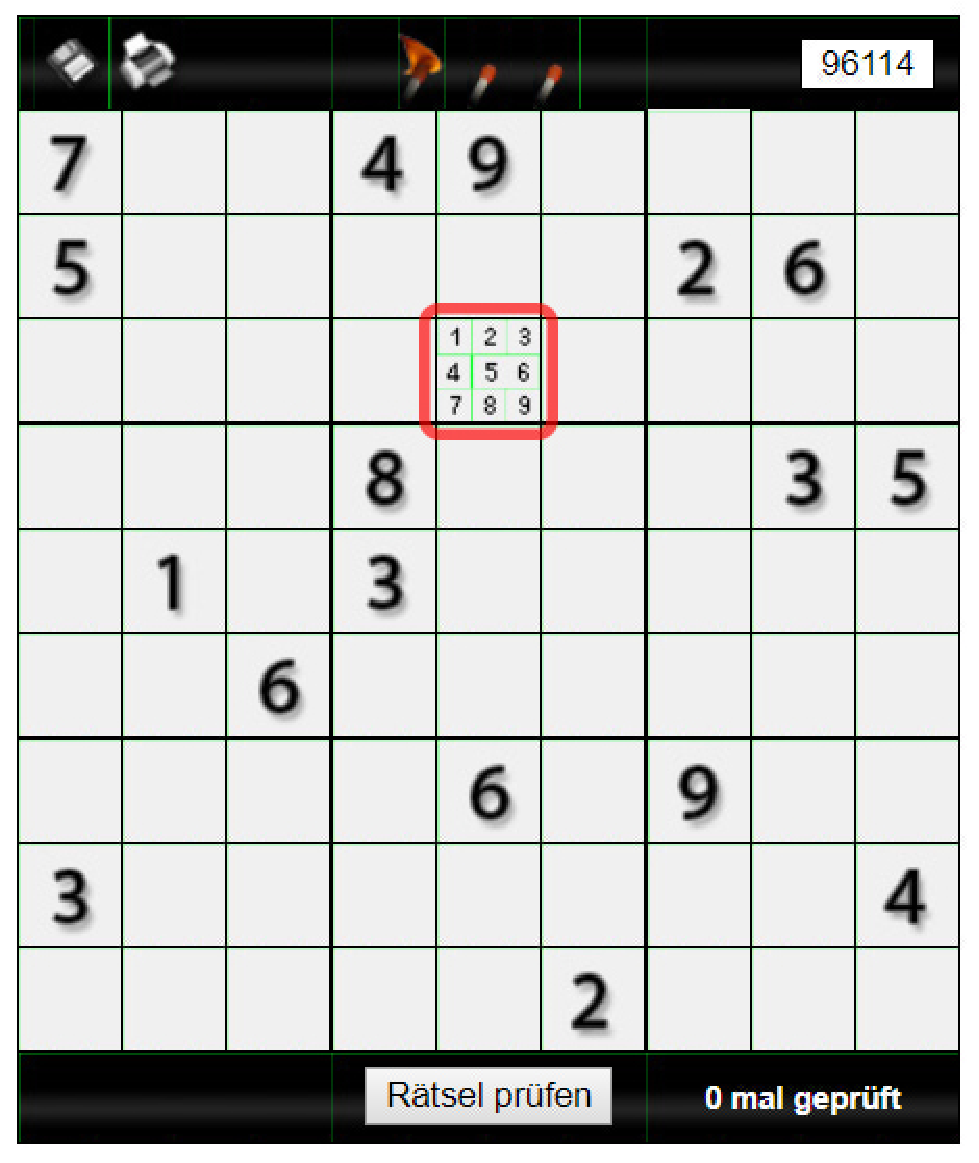
\includegraphics[width=0.33\textwidth]{sudoku1.pdf}
\end{center}
\caption{Notizen in Online-Sudoku}
\end{figure}
\ \\
Natürlich kann man dem Computer nicht einfach sagen, dass er sich Notizen zu machen, sondern muss dem Computer eine Möglichkeit geben diese Informationen zu speichern. Wir haben uns entschieden dazu eine Option von numpy-arrays auszunutzen. In numpy können nämlich drei-dimensionale arrays erstellt werden. Diese haben nicht nur eine Höhe und eine Breite, sondern auch eine Tiefe. Man kann es sich vorstellen als eine Reihe von zwei-dimensionalen arrays die man hintereinander aufgestellt hat. Bei der Ausgabe sieht ein solches drei-dimensionales array etwa so aus: 
\newpage

\begin{verbatim}
import numpy as np

a = np.zeros((3,4,2))
a[1,:,:] = 1
a[2,:,:] = 2
print(a)
>> 
[[[ 0.  0.]
  [ 0.  0.]
  [ 0.  0.]
  [ 0.  0.]]

 [[ 1.  1.]
  [ 1.  1.]
  [ 1.  1.]
  [ 1.  1.]]

 [[ 2.  2.]
  [ 2.  2.]
  [ 2.  2.]
  [ 2.  2.]]]
\end{verbatim}
\ \\
So nutzen wir diese Eigenschaft für unser Sudoku. Das eigentliche Sudoku bildet die 'oberste' Ebene, danach bildet die nächste Ebene, eine Ebene für die Möglichen Felder in denen eine Eins stehen kann, die darauf Folgenden eine für die in denen eine Zwei stehen kann und so weiter. Steht in einem Feld in der dritten Ebene (also die Ebene für die Zweien) eine Zwei, so bedeutet das, dass in dem eigentlichen Feld an dieser Stelle eine Zwei stehen könnte. Steht an der selben Stelle eine Null, so bedeutet das, dass in dem betreffenden Sudoku an dieser Stelle keine Zwei stehen kann. Die Funktion die so ein leeres Sudoku in dem noch alles möglich ist, realisiert, sieht wie folgt aus:  
\ \\
\begin{verbatim}
import numpy as np       

def empty_sudoku():              
    sudoku = np.zeros((10,9,9))
    for i in range(10):
        sudoku[i,:,:] = i
    
    return(sudoku)
\end{verbatim}
\ \\
\newpage
\ \\
\subsubsection{Einträge im Sudoku verändern}
Der nächste Schritt war es, eine Funktion zu schreiben mit der wir Einträge in unserem Sudoku verändern konnten. Das Problem dabei ist allerdings, dass das Setzen einer Zahl im Sudoku Einfluss darauf hat, welche Zahlen in andere Felder des Sudoku kommen können. Nach den Regeln für ein Sudoku darf in jeder Zeile, in jeder Spalte und in jedem 3x3 Kästchen jede Zahl von 1 bis 9 nur einmal auftreten. Somit beeinflusst das Setzen einer Zahl die Möglichkeiten in Folgenden Feldern:
\ \\
\begin{figure}[htbp!]
\begin{center}
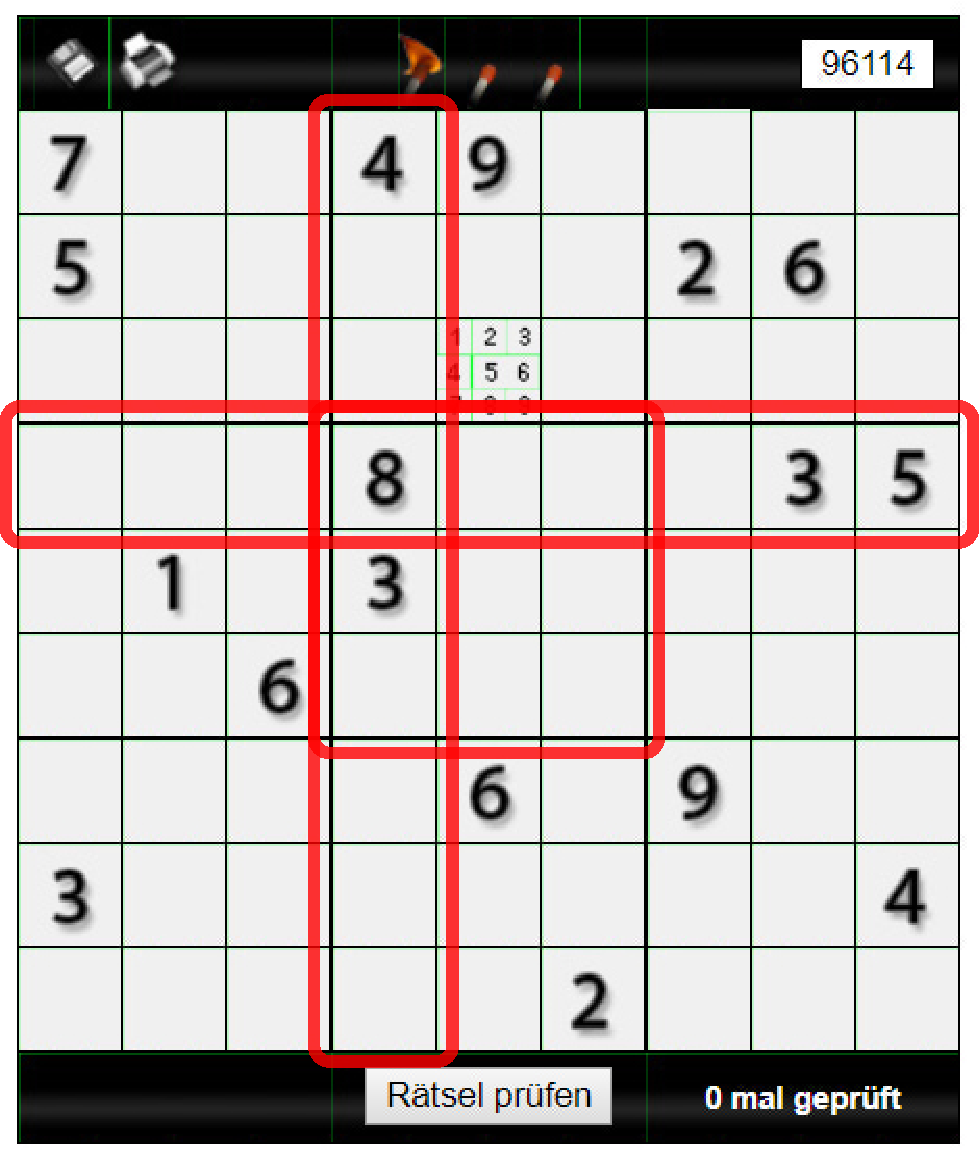
\includegraphics[width=0.33\textwidth]{sudoku2.pdf}
\end{center}
\caption{Felder die Beeinflusst werden}
\end{figure}
\ \\ 
In dem Vorliegenden Beispiel kann, aufgrund der Acht, weder in der vierten Zeile, Spalte oder dem Mittleren 3x3 Kästchen eine Acht stehen. Außerdem kann natürlich auch im Feld in dem die Acht steht, keine andere Zahl mehr stehen. Die Funktion die das Sudoku entsprechend ändert, sieht wie folgt aus:
\ \\
\begin{verbatim}
def clues(sudoku, zahl, x, y):
    x = x - 1                       
    y = y - 1                        
    sudoku[0,y,x] = zahl             
    sudoku[1:,y,x] = 0               
    sudoku[zahl,:,x] = 0             
    sudoku[zahl,y,:] = 0             
    
    if x in [0,1,2]:                 
        if y in [0,1,2]:             
            sudoku[zahl,0:3,0:3] = 0 
        
        elif y in [3,4,5]:
            sudoku[zahl,3:6,0:3] = 0
        
        elif y in [6,7,8]:
            sudoku[zahl,6:9,0:3] = 0
        
    
    elif x in [3,4,5]:
        if y in [0,1,2]:
            sudoku[zahl,0:3,3:6] = 0
        
        elif y in [3,4,5]:
            sudoku[zahl,3:6,3:6] = 0
        
        elif y in [6,7,8]:
            sudoku[zahl,6:9,3:6] = 0
    
    elif x in [6,7,8]:
        if y in [0,1,2]:
            sudoku[zahl,0:3,6:9] = 0
        
        elif y in [3,4,5]:
            sudoku[zahl,3:6,6:9] = 0
        
        elif y in [6,7,8]:
            sudoku[zahl,6:9,6:9] = 0
    
    return(sudoku)
\end{verbatim}
\ \\
Durch diese Funktion wird in das Feld des Sudokus zunächst die gefragten Zahl eingesetzt. Dann wird das Feld auf allen darunterliegenden Ebenen gleich Null gesetzt, da in dieses Feld nun keine andere Zahl mehr eingesetzt werden kann. Dann werden auf der Ebene der Zahl die in das Feld eingesetzt wurde, die Zeile und Spalte in der das Feld liegt, gleich Null gesetzt. In dem Beispiel von zuvor, würde auf der Ebene in der die Möglichkeiten für die Zahl Acht gespeichert sind, also der neunten, die vierte Zeile und die vierte Spalte gleich Null gesetzt. Zuletzt wird identifiziert in welchem 3x3 Feld sich das Feld befindet, dieses wird dann ebenfalls auf der Ebene der Zahl gleich Null gesetzt.\\
Mit dieser Funktion kann nun ein Sudoku wie das aus dem Beispiel erstellt werden.
\ \\
\subsubsection{Ausschluss-Prinzip für ein Feld}
Wir können nun also ein Sudoku, welches wir lösen wollen, eingeben.
Nun ging es daran, einen Lösungsalgorithmus zu entwickeln. Dazu mussten wir uns überlegen, welche Hinreichenden Bedingungen erfüllt sein müssen, damit eine Zahl in das Sudoku eingesetzt werden darf. Zunächst natürlich: Eine Zahl kann eingesetzt werden, wenn diese Zahl die einzige Möglichkeit ist, ein Feld zu füllen. in unserem Algorithmus haben wir diese Bedngung wie folgt umgesetzt:
\ \\
\begin{verbatim}
        for i in range(9):           
            for j in range(9):       
                reihe = sudoku[1:10,i,j]                                     
                pruef = check_list(reihe)      
                if pruef == 1:            
                    sudoku = clues(sudoku,int(reihe[np.argmax(reihe)]),j+1,i+1) 
\end{verbatim}
\ \\
Es wird über alle Felder iteriert und bei jedem Feld alle Möglichkeiten in eine Liste geschrieben. Die Funktion check\_list überprüft dann, wie viele Elemente in der Liste der Möglichkeiten ungleich Null sind. Sollte nur eines der Elemente ungleich Null sein, soll diese Zahl im Sudoku an der entsprechenden Stelle als neuer Hinweis mithilfe der Funktion clues eingefügt werden. Die dabei benutzte Funktion check\_ list ist die folgende:
\ \\
\begin{verbatim}
def check_list(reihe):
    x = 0
    for i in range(9):
        if reihe[i] != 0:
            x = x + 1
    return(x) 
\end{verbatim}
\ \\
\subsubsection{Ausschluss-Prinzip für ein Kästchen}
Die nächste Bedingung die wir implementierten, ist die, dass wenn in einem 3x3 Kästchen eine Zahl nur in einem Kästchen auftauchen kann, dass diese an dieser Stelle in das Sudoku eingesetzt wird. Zur Veranschaulichung: 
\ \\
\begin{figure}[htbp!]
\begin{center}
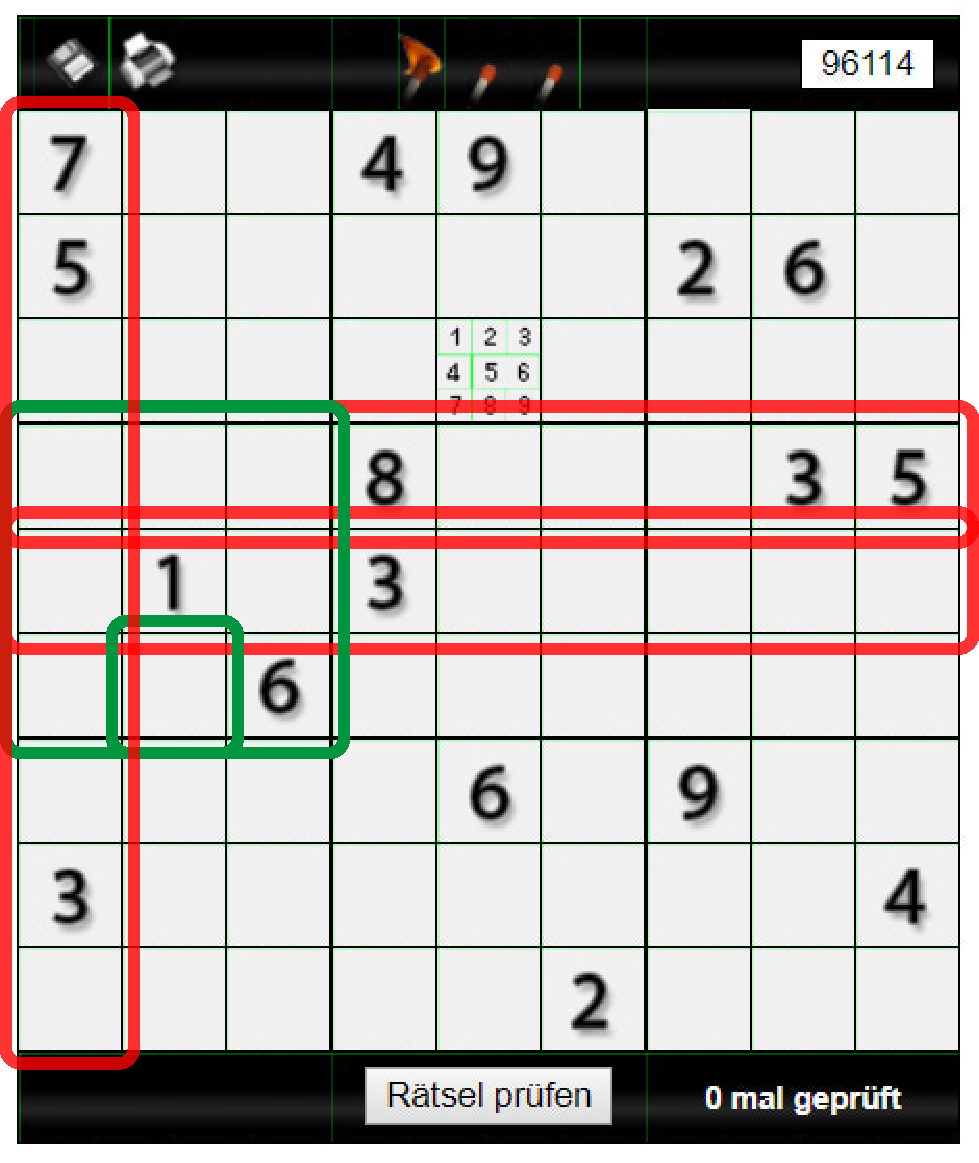
\includegraphics[width=0.33\textwidth]{sudoku3.pdf}
\end{center}
\caption{Zweite Hinreichende Bedingung}
\end{figure}
\ \\ 
In dem großen grünen Feld kann aufgrund der anderen dreien im Sudoku nur das kleine grüne Feld im großen grünen Feld mit der drei besetzt werden. Da eine drei in das große grüne Feld rein muss, können wir die drei in das kleine grüne Feld einsetzen. Der Mechanismus der identifiziert wann so eine Zahl in das Sudoku eingesetzt werden kann, sieht so aus:
\ \\
\begin{verbatim}
        for n in range(1,10):
            for m in range(3):       
                for o in range(3):   
                    square = sudoku[n,3*m:3*(m+1),3*o:3*(o+1)]    
                    pruef = check_square(square)                  
                    if pruef == 1:                           
                        if int(np.argmax(square)) in [0,1,2]:
                            y = 1
                        
                        elif int(np.argmax(square)) in [3,4,5]:
                            y = 2
                        
                        elif int(np.argmax(square)) in [6,7,8]:
                            y = 3
                    
                        if int(np.argmax(square)) in [0,3,6]:
                            x = 1
                        
                        elif int(np.argmax(square)) in [1,4,7]:
                            x = 2
                    
                        elif int(np.argmax(square)) in [2,5,8]:
                            x = 3
                        
                        sudoku = clues(sudoku,n,(x + (3*o)),(y + (3*m)))                        
\end{verbatim}
\ \\
Es wird zunächst über die einzelnen Zahlen-Ebenen iteriert. Innerhalb dieser Zahlen-Ebenen wird dann über die einzelnen 3x3 Kästchen iteriert. Die Möglichkeiten in einem 3x3 Kästchen werden dann in ein array geschrieben, bei welchem mit der check\_ square Funktion überprüft wird, wie viele Elemente in dem array ungleich Null sind.
Sollte nur ein Element ungleich Null sein, wird dieses an der entsprechenden Stelle im Sudoku mit der clues-Funktion eingesetzt.\\
\ \\
\subsubsection{Ausschluss-Prinzip für Zeilen und Spalten}
Einen ähnlichen Mechanismus haben wir dann auch für die Zeilen und Spalten geschrieben. Wie auch zuvor, sollte in einer Zeile oder Spalte eine Zahl nur in einem Feld möglich sein, wird diese dort eingesetzt.
\ \\
\begin{verbatim}
        for n in range(1,10):  
            for m in range(9): 
                zeile = sudoku[n,m,:]  
                pruef_zeile = check_list(zeile) 
                if pruef_zeile == 1:      
                    sudoku = clues(sudoku,n,int(np.argmax(zeile)) + 1,m + 1)  
                    
                spalte = sudoku[n,:,m] 
                pruef_spalte = check_list(spalte)
                if pruef_spalte == 1:     
                    sudoku = clues(sudoku,n,m + 1,int(np.argmax(spalte)) + 1)               
\end{verbatim}
\ \\
Ähnlich wie zuvor wird zunächst über die Zahlen-Ebenen und dann über die Zeilen beziehungsweise Spalten iteriert und jedes mal überprüft, wie viele Elemente in einer Zeile/Spalte ungleich Null sind, sollte es nur eine sein, wird das eine Element an der entsprechenden Stelle eingesetzt.\\
\ \\
\subsubsection{Double-Ausschluss}
Wir versuchten unser Programm in diesem Zustand an dem oben schon mehrmals benutzten Beispiel. Wir mussten jedoch feststellen, dass unser Programm an einem bestimmten Punkt nicht weiter kam.
Wir mussten noch weitere Mechanismen hinzufügen um Sudoku wie das folgende lösen zu können:
\ \\
\begin{figure}[htbp!]
\begin{center}
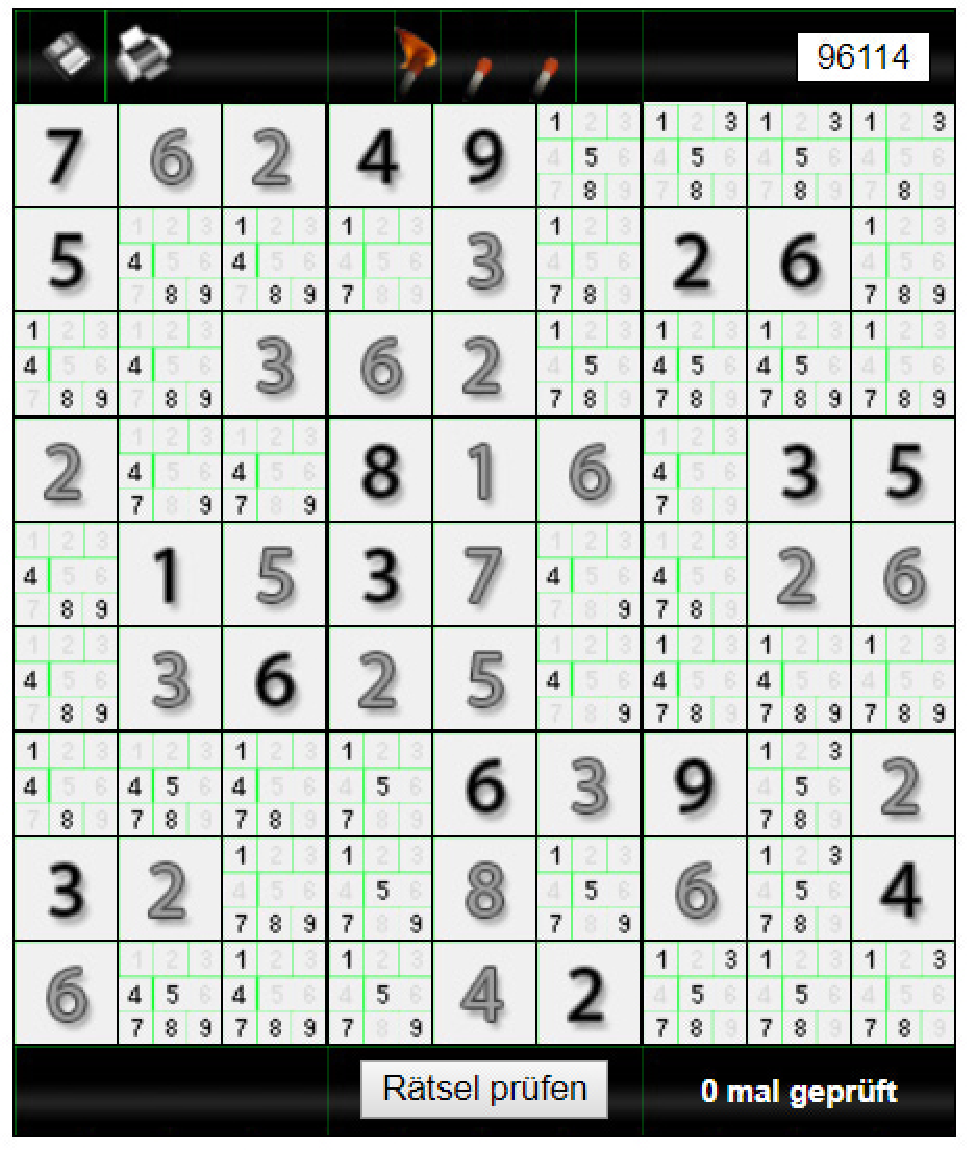
\includegraphics[width=0.33\textwidth]{sudoku4.pdf}
\end{center}
\caption{Problemsituation}
\end{figure}
\ \\ 
\newpage
Um diese Situation zu lösen, müssen wir einer besonderen Konstellation, ganz besondere Beachtung schenken. Diese sieht wie folgt aus: 
\ \\
\begin{figure}[htbp!]
\begin{center}
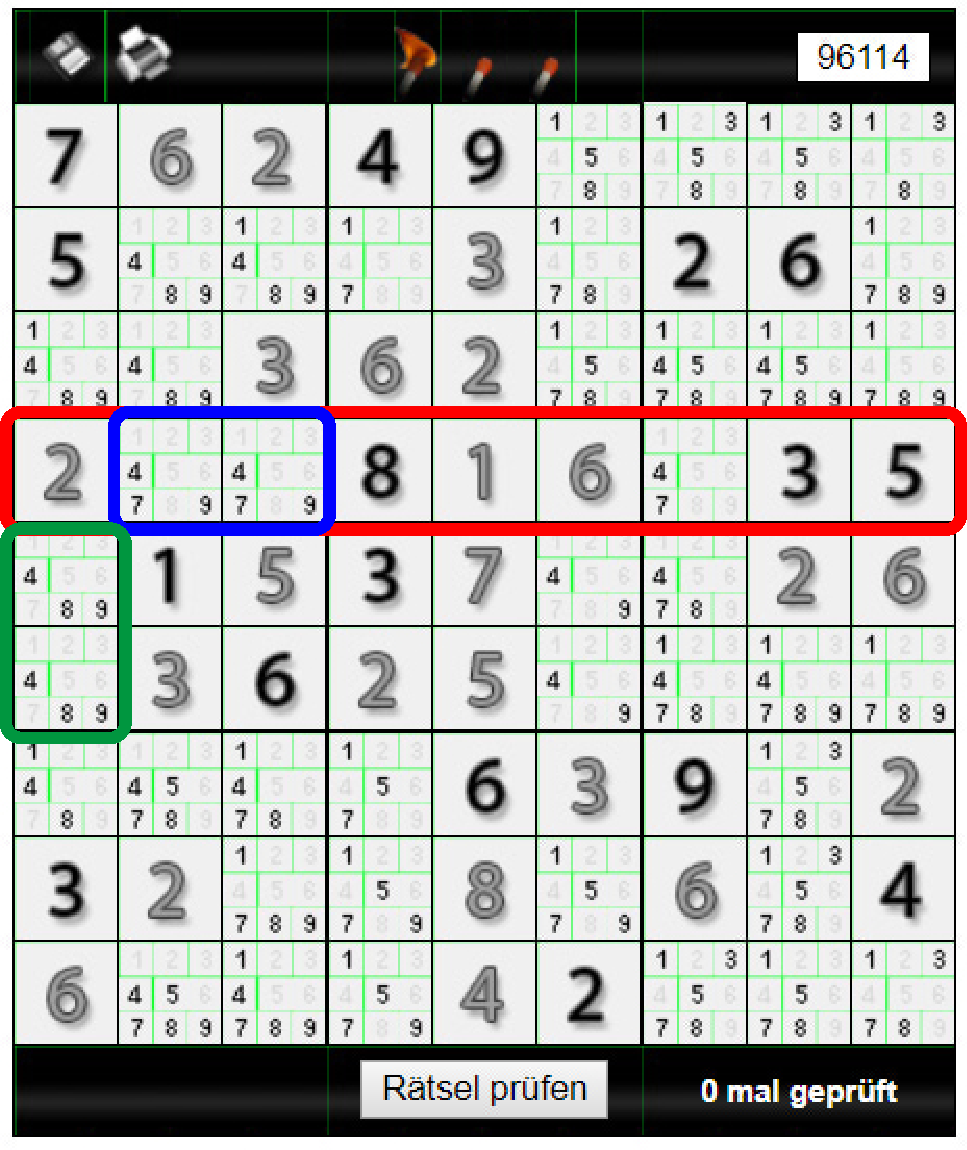
\includegraphics[width=0.33\textwidth]{sudoku5.pdf}
\end{center}
\caption{Problemsituation mit Erläuterung}
\end{figure}
\ \\ 
Betrachten wir die rot umrandete Zeile, fällt auf das noch die Zahl neun fehlt. Des Weiteren fällt uns auf, dass die Neun nur in den Blau umrandeten Feldern sein könnte. Da in der roten Zeile eine Neun sein muss, bedeutet dies, dass in den grünen Feldern die Neun nicht sein kann. Und diese Korrelation ist es, die es ermöglicht das Sudoku zu lösen. Es lässt sich allgemein sagen, dass wenn alle Möglichkeiten eine Zahl zu setzen in einer Zeile oder Spalte nur in einem Kästchen liegen, dann können alle anderen Möglichkeiten diese Zahl in diesem Kästchen zu setzen ignoriert und somit gleich Null gesetzt werden.
Die Programmierung gestaltete sich nun ein wenig anspruchsvoller. Unsere Lösung sieht wie folgt aus:
\ \\
\begin{verbatim}
        if run >= 3:                                   
            for n in range(1,10):                      
                for m in range(9):                   
                    zeile = sudoku[n,m,:]                  
                    pruef_zeile = check_list(zeile)        
                    if pruef_zeile == 2 or pruef_zeile == 3: 
                        doubles = check_double(zeile,pruef_zeile) 
                        if doubles[0] == True:                   
                            if m in [0,3,6]:                                                    
                                sudoku[n,m+1:m+3,doubles[1]*3:(doubles[1]+1)*3] = 0
                            
                            elif m in [1,4,7]:
                                sudoku[n,m-1,doubles[1]*3:(doubles[1]+1)*3] = 0
                                sudoku[n,m+1,doubles[1]*3:(doubles[1]+1)*3] = 0
                            
                            else:
                                sudoku[n,m-2:m,doubles[1]*3:(doubles[1]+1)*3] = 0
                            
                            
                    
                    
                    
                    
                    
                    spalte = sudoku[n,:,m]              
                    pruef_spalte = check_list(spalte)   
                    if pruef_spalte == 2 or pruef_spalte == 3:     
                        doubles = check_double(spalte,pruef_spalte) 
                        if doubles[0] == True:
                            if m in [0,3,6]:                  
                                sudoku[n,doubles[1]*3:(doubles[1]+1)*3,m+1:m+3] = 0
                            
                            elif m in [1,4,7]:
                                sudoku[n,doubles[1]*3:(doubles[1]+1)*3,m-1] = 0
                                sudoku[n,doubles[1]*3:(doubles[1]+1)*3,m+1] = 0
                            
                            else:
                                sudoku[n,doubles[1]*3:(doubles[1]+1)*3,m-2:m] = 0    
\end{verbatim}
\ \\
\subsubsection{Naked-Subset}
Zunächst dachten wir, dass wir damit ein Programm geschrieben hätten, welches alle Sudokus mit einer einzigen Lösung lösen könne. Doch stellte sich nach einigen Versuchen heraus, dass es doch noch einige Sudokus gibt, welche eine einzige Lösung haben, aber unser Programm nicht lösen kann. Durch weitere Recherche fanden wir nun eine weitere Methode, welche zum lösen einiger schwerer Sudokus benötigt wird. Im folgenden erstmal das problematische Sudoku.
\newpage
\ \\
\begin{figure}[htbp!]
\begin{center}
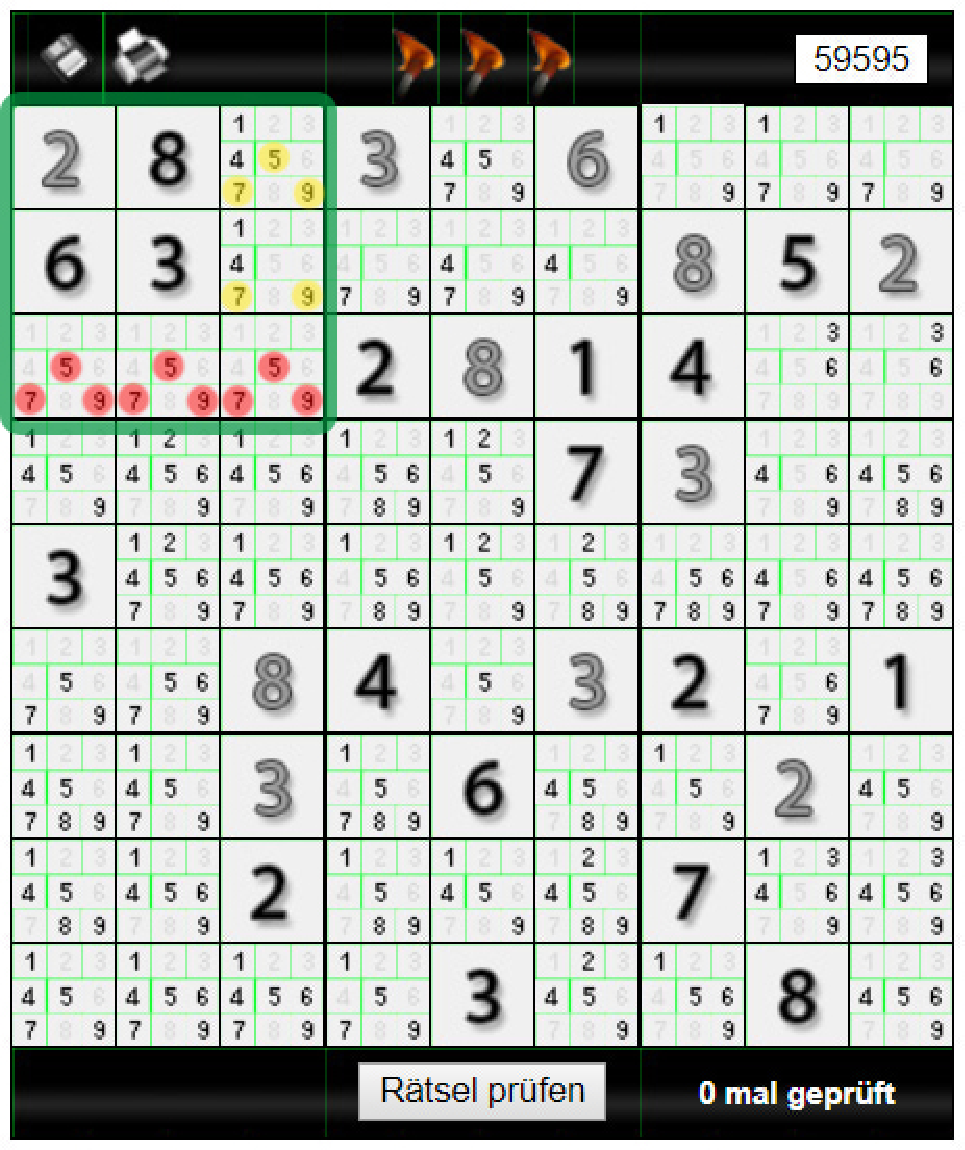
\includegraphics[width=0.33\textwidth]{sudoku6.pdf}
\end{center}
\caption{Naked-Subset}
\end{figure}
\ \\ 
Betrachtet man das grüne 3x3 Kästchen, fällt auf, dass in den unteren drei Feldern nur die rot markierten Möglichkeiten untergebracht werden können. Daraus folgt, dass diese Rot markierten Möglichkeiten auch nur in diesen drei Feldern untergebracht werden können. Somit können die gelb markierten Möglichkeiten eliminiert werden. Der Code der solche Situationen identifiziert sieht wie folgt aus:
\begin{verbatim}
for a in range(3):   
    for b in range(3): 
        square = sudoku[:,a*3:(a+1)*3,b*3:(b+1)*3]  
        for c in range(3):      
            for d in range(3):  
                if square[0,c,d] == 0:              
                    compare = square[:,c,d]         
                    num = check_list(compare[1:10]) 
                    sims = 0                        
                    coor = []                      
                    elem = []                       
                    for i in range(3):              
                        for j in range(3):          
                            if square[0,i,j] == 0:  
                                test = square[:,i,j]
                                if np.array_equal(compare, test) == True: 
                                    sims = sims + 1                       
                                    coor.append((i,j))                    
                                             
                    if num == sims:                    
                        for k in range(10):             
                            if compare[k] != 0:
                                elem.append(compare[k])
                                    
                        for i in range(3):     
                            for j in range(3):
                                if (i,j) not in coor and square[0,i,j] == 0:
                                    for n in elem:                           
                                        sudoku[int(n),int((a*3)+i),int((b*3)+j)] = 0   
\end{verbatim}
\ \\
Er funktioniert nach dem Prinzip, dass zunächst alle 3x3 Kästchen durchgegangen werden, in diesen Kästchen werden alle Felder und ihre Möglichkeiten durchgegangen. und mit allen anderen Feldern im 3x3 Kästchen verglichen. Sollte es Felder mit den gleichen Möglichkeiten gibt, wird gezählt ob die Anzahl der Felder mit der Anzahl der Möglichkeiten übereinstimmen, dann werden diese Möglichkeiten aus den anderen Feldern entfernt.
\ \\
\subsubsection{Force-Chain}
Aber nur mit dieser Funktion ließ sich das problematische Sudoku nicht lösen. Allerdings fanden wir auch keine Methoden um die Möglichkeiten im Sudoku einzuschränken. Wir fanden durch weitere Recherche heraus, dass es Sudokus gibt, bei denen man nur mit konventionellen Methoden nicht weiter kommt, sodass man sogenannte Force-Chains nutzen muss. Dabei sucht man sich ein leeres Feld, welches mit möglichst vielen anderen Feldern in Verbindung steht und welches nur noch zwei bis drei Möglichkeiten besitzt. Dann setzt man in dieses Feld eine der Möglichkeiten ein und versucht das Sudoku zu lösen. Kommt man zu einem Ergebnis, war die Auswahl richtig, kommt man aber zu einem Widerspruch, war die Auswahl wohl falsch und man kann eine der anderen Möglichkeiten probieren. Bei unserem problematischen Sudoku boten sich beispielsweise die folgenden markierten Felder an:
\ \\
\begin{figure}[htbp!]
\begin{center}
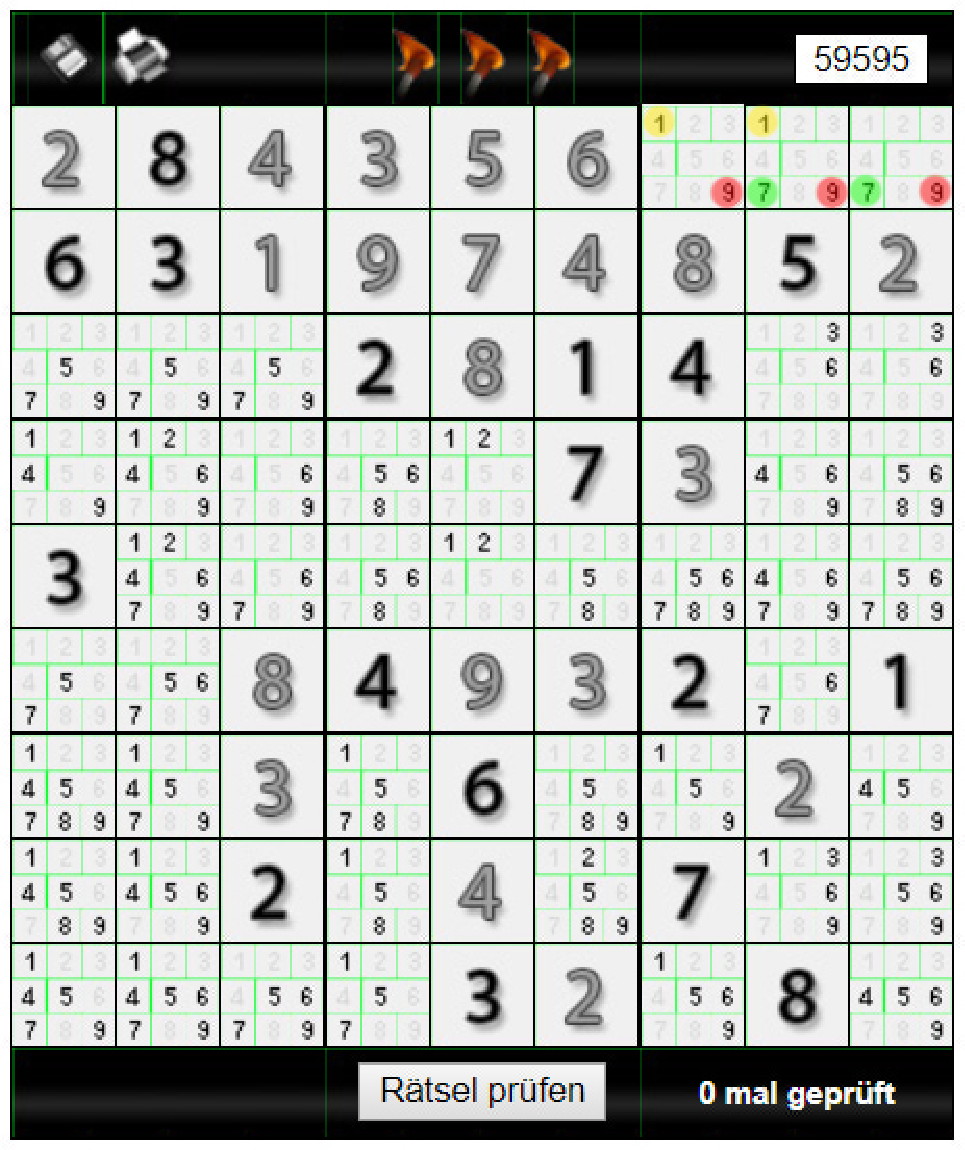
\includegraphics[width=0.33\textwidth]{sudoku7.pdf}
\end{center}
\caption{Force-Chain}
\end{figure}
\ \\ 
Auch hier war die Implementierung etwas problematisch. Die entgültige Lösung nun hier:
\\
\begin{verbatim}
if run >= 2:
    for y in range(9):       
        for x in range(9):            
            if sudoku[0,y,x] == 0:       
                reihe = sudoku[1:,y,x]    
                trys = check_list(reihe) 
                if trys == 2:            
                elem = []                    
                for t in range(9):            
                    if reihe[t] != 0:         
                        elem.append(reihe[t]) 
                                    
                first_try = int(elem[0])      
                second_try = int(elem[1])     
                TE_sudoku = np.copy(sudoku)   
                TE_sudoku = clues(TE_sudoku,first_try,x+1,y+1) 
                result_one = SudokuSolve(TE_sudoku)  
                if result_one[0] == 'Zwei Lösungen': 
                    return(result_one)               
                
                TE_sudoku = np.copy(sudoku)                     
                TE_sudoku = clues(TE_sudoku,second_try,x+1,y+1) 
                result_two = SudokuSolve(TE_sudoku)             
                if result_one[0] == 'Zwei Lösungen' or result_two[0] == 'Zwei Lösungen':
                    return(['Zwei Lösungen',result_two[1]])                                
                elif result_one[0] == result_two[0]:                                     
                    if result_one[0] == 'Eine Lösung':                   
                        if np.array_equal(result_one[1], result_two[1]): 
                            return(result_one)                           
                        else:                                            
                            return('Zwei Lösungen',result_one[1])        
                    elif result_one[0] == 'Keine Lösung':                
                        return(result_one)                               
                            
                elif result_one[0] == 'Eine Lösung' and result_two[0] == 'Keine Lösung': 
                    return(result_one)                                                   
                
                else:                                                                    
                     return(result_two)                                                   
           
    for y in range(9):                 
        for x in range(9):        
            if sudoku[0,y,x] == 0:           
                reihe = sudoku[1:,y,x]       
                trys = check_list(reihe)     
                if trys == 3:               
                    elem = []                     
                    for t in range(9):             
                        if reihe[t] != 0:          
                            elem.append(reihe[t]) 
                                    
                    first_try = int(elem[0])       
                    second_try = int(elem[1])     
                    third_try = int(elem[2])       
                    TE_sudoku = np.copy(sudoku)    
                    TE_sudoku = clues(TE_sudoku,first_try,x+1,y+1)  
                    result_one = SudokuSolve(TE_sudoku)   
                    if result_one[0] == 'Zwei Lösungen':  
                        return(result_one)                
                    
                    TE_sudoku = np.copy(sudoku)                    
                    TE_sudoku = clues(TE_sudoku,second_try,x+1,y+1) 
                    result_two = SudokuSolve(TE_sudoku)            
                    if result_two[0] == 'Zwei Lösungen':  
                        return(result_two)               
                                                
                    TE_sudoku = np.copy(sudoku)                   
                    TE_sudoku = clues(TE_sudoku,third_try,x+1,y+1) 
                    result_three = SudokuSolve(TE_sudoku)         
                    results = [result_one[0], result_two[0], result_three[0]] 
                    ones = []                                                 
                    if 'Zwei Lösungen' in results:                             
                        if result_one[0] == 'Zwei Lösungen':                  
                            return(['Zwei Lösungen',result_one[1]])           
                                
                        elif result_two[0] == 'Zwei Lösungen':
                            return(['Zwei Lösungen',result_two[1]])
                                
                        else:
                            return(['Zwei Lösungen',result_three[1]])
                                        
                    elif 'Eine Lösung' in results:                            
                        for n in range(2):                                    
                            if results[n] == 'Eine Lösung':                   
                                ones.append(n)                                
                        
                        if len(ones) == 1:                                    
                            if ones[0] == 0:                                  
                                return(result_one)                            
                            
                            elif ones[0] == 1:                                
                                return(result_two)                            
                            else:                                             
                                return(result_three)
                                
                        elif len(ones) == 2:
                            if 0 in ones:
                                if 1 in ones:
                                    if np.array_equal(result_one[1], result_two[1]) == True:
                                        return(result_one)
                                    
                                    else:
                                        return(['Zwei Lösungen',result_one[1]])
                                else:
                                    if np.array_equal(result_one[1], result_three[1]) == True:
                                        return(result_one)
                                    else:
                                        return(['Zwei Lösungen',result_one[1]])
                            else:
                                if np.array_equal(result_two[1], result_three[1]) == True:
                                    return(result_two)
                                else:
                                    return(['Zwei Lösungen',result_two[1]])
                                        
                        else:
                            if np.array_equal(result_one[1], result_two[1]) == True:
                                if np.array_equal(result_one[1], result_three[1]) == True:
                                    return(result_one)
                                else:
                                    return(['Zwei Lösungen',result_one[1]])
                                        
                            else:
                                return(['Zwei Lösungen',result_one[1]])
                                    
                    else: 
                        return(result_one)
                            
                            
    return(['Zwei Lösungen',sudoku])  
\end{verbatim}
\ \\
Wie dieser Abschnitt funktioniert ist etwas komplizierter und wird auch nochmal im Programmcode mit Kommentaren erklärt.
Hier nun ein kurzer Überblick über seine Funktion.
Die Methodik der Force-Chain soll erst eingesetzt werden, wenn alle anderen Möglichkeiten ausgeschöpft sind, deshalb beginnt dieser Abschnitt, mit der Bedingung, dass run größer oder gleich zwei ist, das Programm also im zweiten Durchlauf ohne Veränderung des Sudokus ist. Falls diese Bedingung erfüllt ist, sucht das Programm zunächst nach einem leeren Feld welches nur noch zwei offene Möglichkeiten besitzt. Ist ein solches Feld gefunden, wird in eine Kopie des Orginal-Sudokus die erste der beiden Möglichkeiten eingesetzt und auf die Lösungsfunktion rekursiv zugegriffen, um das Sudoku mit diesen zusätzlichen Informationen zu lösen. Sollte nun das Ergebnis sein, dass das Sudoku zwei oder mehr Lösungen hat, wird dieses auch zurückgegeben. Ist das Ergebnis jedoch, dass das Sudoku eine oder keine Lösung hat, kann das Einsetzen der anderen Möglichkeit noch zu einem anderen Ergebnis führen. So wird auch die andere Möglichkeit eingesetzt und gelöst. Zuletzt werden die Ergebnisse verglichen. Sollte eines der Ergebnisse sein, dass es zwei oder mehr mögliche Lösungen gibt, wird dies, sowie eine mögliche Lösung zurückgegeben.
Sind beide Ergebnisse, dass es eine einzige Lösung gibt, so werden die Ergebnisse verglichen, sollten sie gleich sein, wird das Ergebnis, sowie die Information, dass die Lösung einzigartig ist, zurückgegeben. Wenn sie nicht gleich sind, wird zurückgegeben, dass es zwei Lösungen gibt, sowie eine der Lösungen. Sollte nur eine der beiden Ergebnisse eine Lösung sein, so wird diese zurückgegeben, sollte keines der beiden Ergebnisse eine Lösung sein, wird zurückgegeben, dass es keine Lösung gibt. Nun ist dies aber nicht der einzige Teil der Force-Chain.
Sollte der unwahrscheinliche Fall eintreten, dass es kein leeres Feld mit zwei oder weniger Möglichkeiten gibt, wird ein Feld mit drei Möglichkeiten gesucht und das gesamte Prozedere ähnlich zu dem Fall mit zwei Möglichkeiten durchgeführt. Wenn es kein Feld mit drei oder weniger Möglichkeiten gibt, bedeutet das, dass das Sudoku mit hoher Wahrscheinlichkeit weniger als siebzehn besetzte Felder hat und somit zwei oder mehr Lösungen hat. Aus diesem Grund haben wir uns entschieden, in so einem Fall einfach ausgeben zu lassen, dass das Sudoku zwei oder mehr Lösungen hat. Somit haben wir ein Programm, welches in jedem Fall ein Ergebnis liefert und damit unser erstes Ziel erfüllt.

\newpage
\subsection{Gelöste Rätsel}
Hier nun eine Liste von Sudokus mit denen wir unser Programm  überprüft haben. Zum Zwecke der Wiederholbarkeit, haben wir Sudokus von der Internet-Seite http://www.sudoku17.de . Dort hat jedes Sudoku eine eigene Nummer, mit der es immer wieder aufgerufen werden kann. So stellen wir hier eine Liste der Nummern der Sudokus auf, an denen wir unser Programm getestet haben.
\begin{itemize}
\item 71230
\item 7315
\item 59595
\item 67806
\item 60216
\item 59415
\item 79393
\item 59818
\end{itemize}
\newpage

\section{Sudoku-Generator}
Nachdem wir uns zuvor mit dem Lösen von Sudokus beschäftigt haben,  untersuchen wir nun verschiedene Arten Sudokus zu generieren. Zum einen die Variante, in ein leeres Sudoku zufällig Hinweise einzusetzen und zum anderen, aus einem bereits gelösten Sudoku zufällig Zahlen wegzunehmen bis die gewünschte Zahl an Hinweisen erreicht ist. Besonderes Augenmerk richten wir bei unserer Untersuchung auf die Lösbarkeit der generierten Sudokus. Vorarbeit wurde in dieser Hinsicht schon geleistet, da Gary McGuire, Bastian Tugemann und Gilles Civario 2013 in ihrer Arbeit '"There is no 16-Clue Sudoku: Solving the Sudoku Minimum Number of Clues Problem via Hitting Set Enumeration'" bewiesen haben, dass alle lösbaren Sudokus mit 16 oder weniger Hinweisen mindestens zwei Lösungen haben. Das beschränkt die Hinweiszahlen die wir untersuchen müssen auf 17 bis 81 Hinweise.

\subsection{Generierungsprozesse und Experimente}
\subsubsection{Generierung vollständiger Sudokus}
Zunächst befassten wir uns mit der Generierung von vollständigen Sudokus.
Hier war unsere erste Idee, der Reihe nach zufällig Zahlen in das Sudoku Feld einzusetzen bis das Einsetzen weiterer Zahlen zu Widersprüchen führen würde, oder das Sudoku vollständig ist. Sollte es zu Widersprüchen kommen, sollte die Funktion zurückgehen und bereits gesetzte Zahlen neu wählen, bis alle Felder gefüllt sind. Dies erwies sich jedoch in der Umsetzung schwierig. Als zweckdienlicher stellte sich das Verfahren heraus, Zahlen nach gegeben Möglichkeiten einzusetzen und Widersprüche zu überspringen. Erzeugt man so nur genug Sudokus, werden auch schnell einige Auftreten, die keine Widersprüche aufweisen und somit als vollständige Sudokus verwendet werden können. Der Code der dies bewerkstelligt sieht so aus:
\\
\begin{verbatim}
def mkAnswer(sudoku):
    for Y in range(9):
        for X in range(9):
            if sudoku[Y,X] == 0:
                sudoku = setNumber(X,Y,sudoku)

            
    return(sudoku)



def setNumber(X,Y,sudoku):
    possibilitys = mklst(X,Y,sudoku)
    P = len(possibilitys)
    if P > 0:
        sudoku[Y,X] = np.random.choice(possibilitys,1)

    return(sudoku)











def mklst(X,Y,sudoku):
    lst = [1,2,3,4,5,6,7,8,9]
    zeile = sudoku[Y,0:9] 
    spalte = sudoku[0:9,X]
    
    if Y in [0,1,2]:
        if X in [0,1,2]:
            square = sudoku[0:3,0:3]
            
        elif X in [3,4,5]:
            square = sudoku[0:3,3:6]
            
        elif X in [6,7,8]:
            square = sudoku[0:3,6:9]
        
    elif Y in [3,4,5]:
        if X in [0,1,2]:
            square = sudoku[3:6,0:3]
        
        elif X in [3,4,5]:
            square = sudoku[3:6,3:6]
            
        elif X in [6,7,8]:
            square = sudoku[3:6,6:9]
        
    elif Y in [6,7,8]:
        if X in [0,1,2]:
            square = sudoku[6:9,0:3]
            
        elif X in [3,4,5]:
            square = sudoku[6:9,3:6]
            
        elif X in [6,7,8]:
            square = sudoku[6:9,6:9]
    
    rechteck = np.reshape(square,9)
    
    for s in spalte:
        if s in lst:
            lst.remove(s)
    
    for z in zeile:
        if z in lst:
            lst.remove(z)
            
    for r in rechteck:
        if r in lst:
            lst.remove(r)
            
    return(lst)
  
  
    
solved = False
while solved != True:
    sudoku = np.zeros((9,9))
    sudoku = mkAnswer(sudoku)
    solved = check_sudoku(sudoku)
\end{verbatim}
\ \\
Zunächst die mkAnswer-Funktion: Diese gibt das Sudoku aus. Es wird über alle Felder eines leeren Sudokus iteriert und mit der Funktion setNumber in die leeren Felder Zahlen eingesetzt. Bei der setNumbers Funktion wird zunächst eine Liste der Möglichen Zahlen, die in ein Feld kommen kann, mit Hilfe der mklst Funktion erstellt. Sollte die Liste nicht leer sein, wird zufällig eine der Möglichkeiten eingesetzt. Wenn die Liste Leer ist, bleibt in dem Feld eine Null.
Bei der mklst Funktion wird zunächst eine vollständige Liste der möglichen Zahlen erstellt. Aus dieser werden dann die Zahlen entfernt, wenn sie in der Zeile, Spalte oder dem 3x3 Kästchen schon einmal vorkommen.
Zuletzt werden auf diese Variante Sudokus erstellt, bis das Programm ein Sudoku erstellt hat, in dem keine Nullen mehr sind. Überprüft wird dies mit der check\_sudoku Funktion die schon bei unserem Sudoku-Lösungsprogramm zum Einsatz kam. Am Ende hat man eine vollständig ausgefülltes Sudoku.
\ \\
\ \\
\subsubsection{Test 1: Sudoku generieren durch zufälliges herausnehmen von Zahlen}
Nachdem wir nun ein vollständiges Sudoku haben, versuchen wir nun durch zufälliges herausnehmen von Zahlen aus ebendiesem ein Sudoku-Puzzle zu erstellen.
Für unseren Test haben wir unser Programm für alle möglichen Hinweiszahlen von 17 bis 81 je 500 Sudoku-Puzzle (also Sudokus in denen nur die Hinweise stehen) generiert und auf ihre Lösbarkeit getestet. Mögliche Ergebnisse waren dabei, ''keine Lösung'', ''eine einzige Lösung'' oder ''zwei oder mehr Lösungen''.
Der Code für diesen Test ist folgender:
\ \\
\begin{verbatim}
def make_sudoku(N):
    pos = [0,1,2,3,4,5,6,7,8]
    z = 0
    solved = False
    while solved != True:
        sudoku = np.zeros((9,9))
        sudoku = mkAnswer(sudoku)
        solved = check_sudokuG(sudoku)
    
    x = check_list(sudoku.reshape(81))
    while x != N:
        i = np.random.choice(pos)
        j = np.random.choice(pos)
        sudoku[i,j] = 0
        x = check_list(sudoku.reshape(81))
    
    return(sudoku)








    
ergebnisse = []                       
for N in range(17,82):                

    null = 0                         
    eins = 0                          
    zwei = 0                          
                              
    for n in range(500):              
        quest = make_sudoku(N)        
        sudoku = empty_sudoku()                                    
        for y in range(1,10):                                      
            for x in range(1,10):                                  
                if quest[y-1,x-1] != 0:                            
                    sudoku = clues(sudoku,int(quest[y-1,x-1]),x,y) 
        

        SUSO = SudokuSolve(sudoku)                                      
        
        if SUSO[0] == 'Keine Lösung':           
            null = null + 1                     
                                                
        elif SUSO[0] == 'Zwei Lösungen':        
            zwei = zwei + 1                     
                                                
        elif SUSO[0] == 'Eine Lösung':          
            eins = eins + 1                     
                         
    ergebnisse.append([null,eins,zwei]) 
            
\end{verbatim}
Die Funktion make\_sudoku erstellt wie zuvor beschrieben ein Sudoku mit N Hinweisen und der darauffolgende Code testet die einzelnen Sudokus auf ihre Lösbarkeit. Das Ergebnis ist in der folgenden Tabelle festgehalten.
\newpage

\ \\
\begin{table}[htbp!]
\scriptsize
\begin{center}
\begin{tabular}[htbp!]{|*{3}{c|}}
\hline 
Hinweise & Eine Loesung & Zwei oder mehr Loesungen\\ \hline 
17 & 0 & 500 \\ \hline 
 18 & 0 & 500 \\ \hline 
 19 & 0 & 500 \\ \hline 
 20 & 0 & 500 \\ \hline 
 21 & 0 & 500 \\ \hline 
 22 & 0 & 500 \\ \hline 
 23 & 0 & 500 \\ \hline 
 24 & 0 & 500 \\ \hline 
 25 & 0 & 500 \\ \hline 
 26 & 0 & 500 \\ \hline 
 27 & 1 & 499 \\ \hline 
 28 & 2 & 498 \\ \hline 
 29 & 1 & 499 \\ \hline 
 30 & 6 & 494 \\ \hline 
 31 & 12 & 488 \\ \hline 
 32 & 19 & 481 \\ \hline 
 33 & 32 & 468 \\ \hline 
 34 & 42 & 458 \\ \hline 
 35 & 56 & 444 \\ \hline 
 36 & 72 & 428 \\ \hline 
 37 & 110 & 390 \\ \hline 
 38 & 133 & 367 \\ \hline 
 39 & 139 & 361 \\ \hline 
 40 & 155 & 345 \\ \hline 
 41 & 192 & 308 \\ \hline 
 42 & 194 & 306 \\ \hline 
 43 & 261 & 239 \\ \hline 
 44 & 258 & 242 \\ \hline 
 45 & 281 & 219 \\ \hline 
 46 & 304 & 196 \\ \hline 
 47 & 337 & 163 \\ \hline 
 48 & 350 & 150 \\ \hline 
 49 & 390 & 110 \\ \hline 
 50 & 383 & 117 \\ \hline 
 51 & 409 & 91 \\ \hline 
 52 & 415 & 85 \\ \hline 
 53 & 430 & 70 \\ \hline 
 54 & 432 & 68 \\ \hline 
 55 & 437 & 63 \\ \hline 
 56 & 455 & 45 \\ \hline 
 57 & 455 & 45 \\ \hline 
 58 & 476 & 24 \\ \hline 
 59 & 472 & 28 \\ \hline 
 60 & 481 & 19 \\ \hline 
 61 & 484 & 16 \\ \hline 
 62 & 487 & 13 \\ \hline 
 63 & 485 & 15 \\ \hline 
 64 & 493 & 7 \\ \hline 
 65 & 494 & 6 \\ \hline 
 66 & 496 & 4 \\ \hline 
 67 & 497 & 3 \\ \hline 
 68 & 498 & 2 \\ \hline 
 69 & 498 & 2 \\ \hline 
 70 & 497 & 3 \\ \hline 
 71 & 499 & 1 \\ \hline 
 72 & 499 & 1 \\ \hline 
 73 & 500 & 0 \\ \hline 
 74 & 500 & 0 \\ \hline 
 75 & 500 & 0 \\ \hline 
 76 & 500 & 0 \\ \hline 
 77 & 500 & 0 \\ \hline 
 78 & 500 & 0 \\ \hline 
 79 & 500 & 0 \\ \hline 
 80 & 500 & 0 \\ \hline 
 81 & 500 & 0 \\ \hline 
 \end{tabular}
 \end{center}
 \caption{Test1} 
\end{table} 
\ \\
Die folgende Graphische Darstellung zeigt, wie sich die Wahrscheinlichkeiten ein Sudoku mit einer einzigen Lösung und ein Sudoku mit zwei oder mehr Lösungen zu generieren mit zunehmender Anzahl verhalten.
\ \\
\begin{figure}[htbp!]
\begin{center}
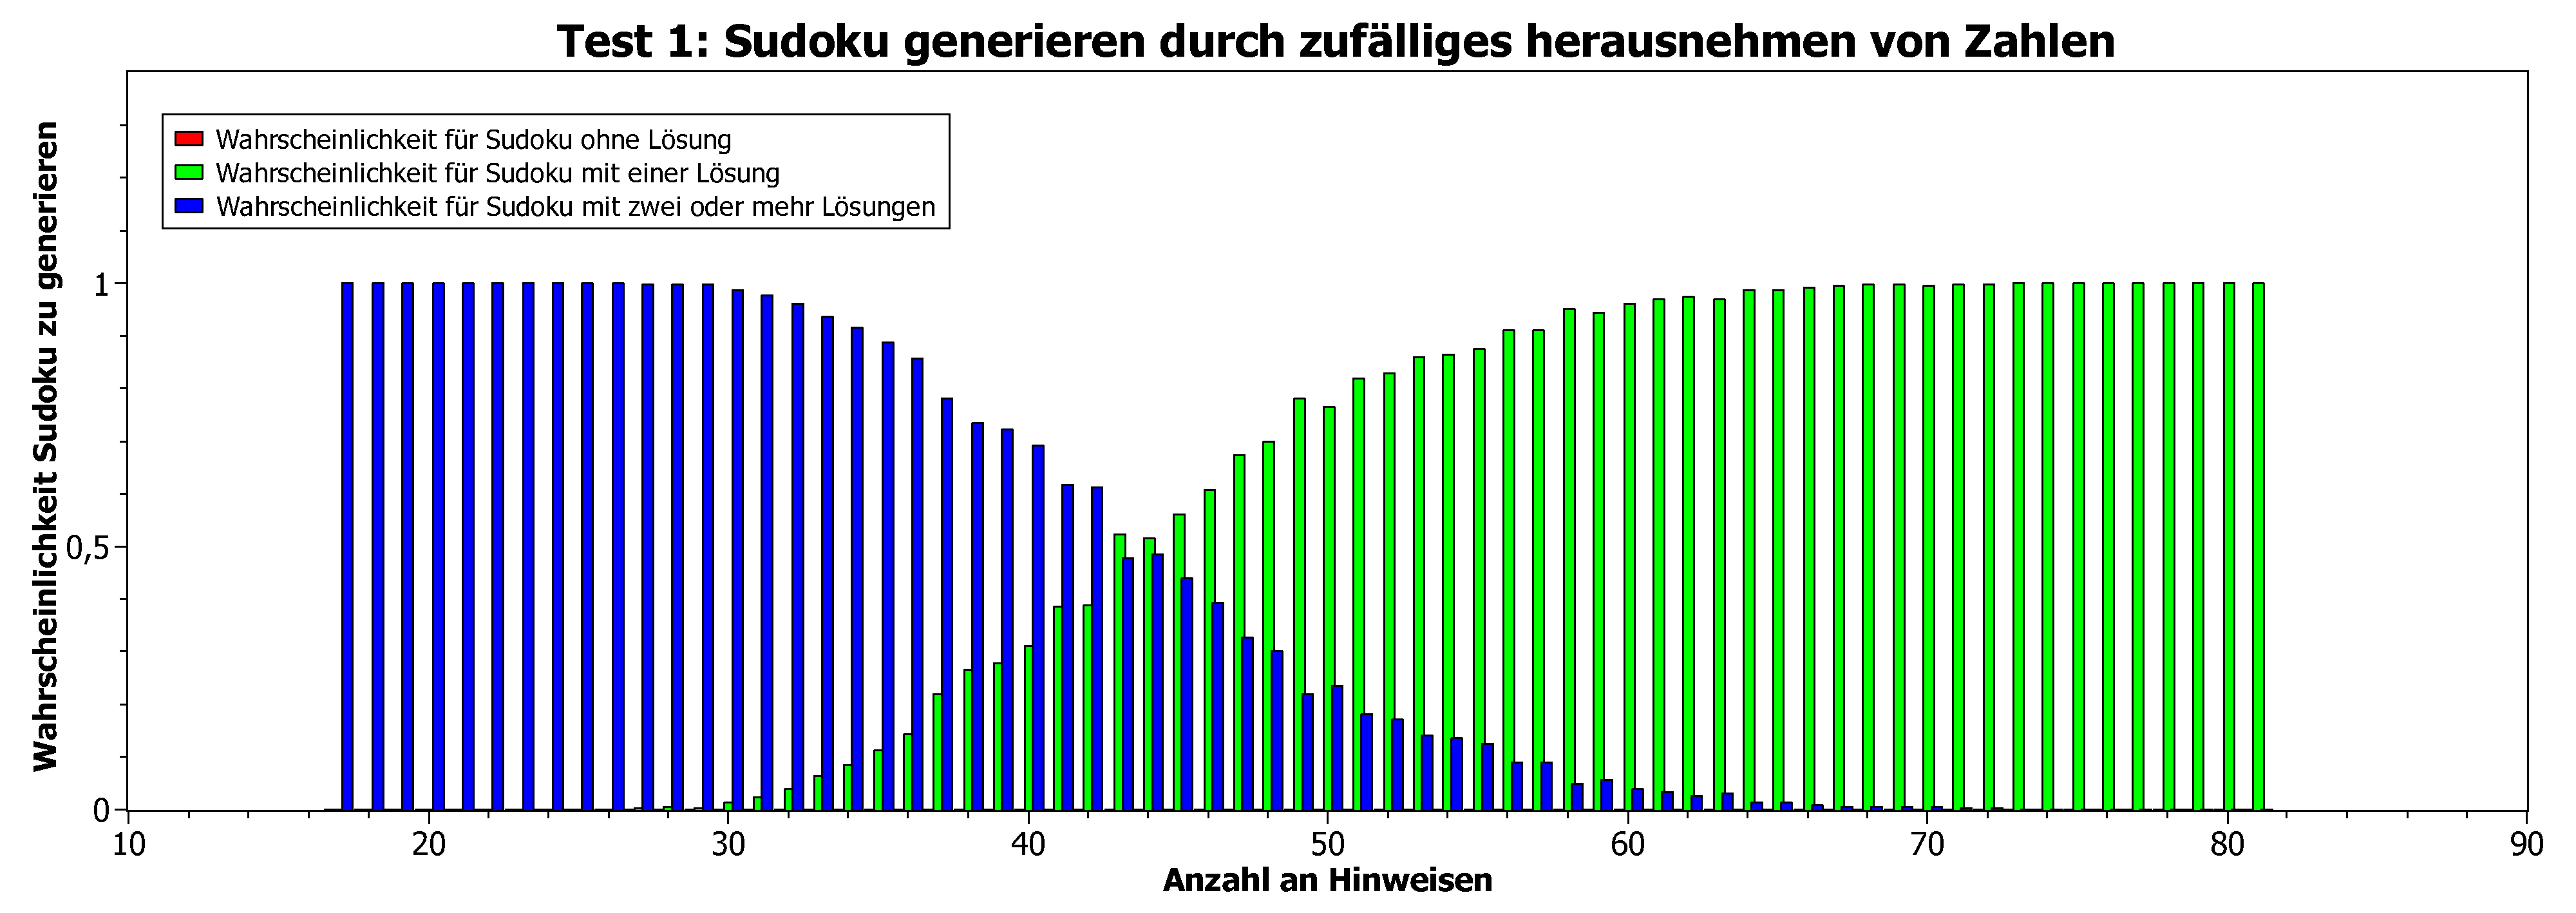
\includegraphics[width=1\textwidth]{Test1ABB.pdf}
\end{center}
\caption{Wahrscheinlichkeiten Sudokus bestimmter Lösbarkeit zu generieren}
\end{figure}
\ \\ 
Die Auswertung zeigt ganz klar die Stärken dieser Methode auf. Zum einen sind alle Sudokus die wir generieren entweder einfach oder mehrfach lösbar, es kann aber nie passieren, dass eines unserer Sudokus keine Lösung aufweist. Des Weiteren fällt auf, dass die Anzahl von Sudokus mit einer einzigen Lösung nahe zu logistisch zunimmt. So, müssen wir nicht allzu lange suchen, wenn wir ein einzigartig lösbares Sudoku mit 30 oder mehr Hinweisen generieren wollen.
Allerdings bedeutet das auch, dass wir signifikant länger suchen müssen, wenn es darum geht ein Sudoku mit 20 oder weniger Hinweisen zu finden.
 
\subsubsection{Test 2: Sudoku generieren durch zufälliges Hinzufügen ohne Regel}
\ \\
\begin{verbatim}
ergebnisse = []                       
pos = [1,2,3,4,5,6,7,8,9]             
for N in range(17,82):                

    null = 0                          
    eins = 0                          
    zwei = 0                          
    
    print(N)                          
    for n in range(500):              
        sudoku = empty_sudoku()       
        c = 0                         
        while c < N:                                     
            x = np.random.choice(pos) - 1                
            y = np.random.choice(pos) - 1                
            z = np.random.choice(pos)                    
            if sudoku[0,y,x] == 0:                       
                sudoku = clues(sudoku,z,x + 1,y + 1)     
                c = c + 1                                
        
        SUSO = SudokuSolve(sudoku)         
        
        if SUSO[0] == 'Keine Lösung':     
            null = null + 1               
                                           
        elif SUSO[0] == 'Zwei Lösungen':   
            zwei = zwei + 1                
                                           
        elif SUSO[0] == 'Eine Lösung':     
            eins = eins + 1                
            
    ergebnisse.append([null,eins,zwei]) 
\end{verbatim}
\ \\

\subsubsection{Test 3: Sudoku generieren durch zufälliges Hinzufügen mit mäßigen Regel}
\ \\
\begin{verbatim}
ergebnisse = []                          
korr = [0,1,2,3,4,5,6,7,8]               
pos = [1,2,3,4,5,6,7,8,9]                
for N in range(17,82):                   

    null = 0                             
    eins = 0                             
    zwei = 0                             
    
    for n in range(500):                 
        sudoku = empty_sudoku()          
        c = 0                            
        while c < N:                                  
            x = np.random.choice(korr)                
            y = np.random.choice(korr)                
            z = np.random.choice(pos)                 
            if sudoku[0,y,x] == 0:                    
                sudoku = clues(sudoku,z,x + 1,y + 1)  
                c = c + 1                             
                if c < 8:                             
                    pos.remove(z)                     
                
                else:                                 
                    pos = [1,2,3,4,5,6,7,8,9]         
                    
        
        SUSO = SudokuSolve(sudoku)         
        if SUSO[0] == 'Keine Lösung':      
            null = null + 1                
        elif SUSO[0] == 'Zwei Lösungen':  
            zwei = zwei + 1                                               
        elif SUSO[0] == 'Eine Lösung':     
            eins = eins + 1                
    
    ergebnisse.append([null,eins,zwei])    
\end{verbatim}
\ \\

\subsubsection{Test 4: Sudoku generieren durch zufälliges Hinzufügen mit strengen Regel}
\ \\
\begin{verbatim}
ergebnisse = []                          
korr = [0,1,2,3,4,5,6,7,8]               
pos = [1,2,3,4,5,6,7,8,9]                
for N in range(17,82):                   

    null = 0                             
    eins = 0                             
    zwei = 0                             
    
    for n in range(500):                 
        sudoku = empty_sudoku()          
        c = 0                            
        while c < N:                                  
            x = np.random.choice(korr)                
            y = np.random.choice(korr)                
            z = np.random.choice(pos)                
            pruef = mklstP(x,y,sudoku)                
            if sudoku[0,y,x] == 0 and z in pruef:     
                sudoku = clues(sudoku,z,x + 1,y + 1)  
                c = c + 1                             
                if c < 8:                             
                    pos.remove(z)                     
                                                      
                else:                                 
                    pos = [1,2,3,4,5,6,7,8,9]         
                    
            elif sudoku[0,y,x] == 0 and pruef == []:  
                sudoku = empty_sudoku()               
                c = 0                                 

        SUSO = SudokuSolve(sudoku)         
        if SUSO[0] == 'Keine Lösung':      
            null = null + 1                
                                           
        elif SUSO[0] == 'Zwei Lösungen':   
            zwei = zwei + 1                
                                           
        elif SUSO[0] == 'Eine Lösung':     
            eins = eins + 1                
    
    ergebnisse.append([null,eins,zwei])    
\end{verbatim}
\ \\

\subsubsection{Test 5: Sudoku generieren durch zufälliges herausnehmen von Zahlen mit Regeln}
\ \\
\begin{verbatim}
ergebnisse = []                       # Liste der Ergenisse für die einzelnen Hinweiszahlen 
for N in range(17,82):                # Es wird ueber alle moeglichen Hinweiszahlen iteriert 

    null = 0                          # Diese Variable speichert die Anzahl an nicht loesbaren Sudokus
    eins = 0                          # Diese Variable speichert die Anzahl an einzigartig loesbaren Sudokus
    zwei = 0                          # Diese Variable speichert die Anzahl an verschieden loesbaren Sudokus
    
    print(N)                          # gibt die Zahl der Ausgangshinweise aus
    for n in range(500):              # erstellt und ueberprueft 500 Sudokus
        quest = make_uas_sudoku(N)        # erstellt das Sudoku durch zufaelliges wegnehmen aus vollstaendigen Sudokus
        
        sudoku = empty_sudoku()                                    # macht aus dem erstellten Sudoku
        for y in range(1,10):                                      # eines welches fuer den Loeser 
            for x in range(1,10):                                  # passend ist.
                if quest[y-1,x-1] != 0:                            # 
                    sudoku = clues(sudoku,int(quest[y-1,x-1]),x,y) # 
        

        SUSO = SudokuSolve(sudoku)         # Loest Sudoku
        print(n,SUSO[0])                   # gibt Loesbarkeit des Sudokus aus
        
        if SUSO[0] == 'Keine Lösung':      # Loesbarkeit des Sudokus wird verglichen und  
            null = null + 1                # Variablen werden veraendert
                                           #
        elif SUSO[0] == 'Zwei Lösungen':   #
            zwei = zwei + 1                #
                                           #
        elif SUSO[0] == 'Eine Lösung':     #
            eins = eins + 1                #
    
    print([null,eins,zwei])                # gibt Loesbarkeiten fuer Hinweiszahl aus
    ergebnisse.append([null,eins,zwei])    # erweitert Liste der Ergebnisse

print(ergebnisse)
\end{verbatim}
\ \\

\subsection{Generator zum erstellen von Sudokus}
\ \\
\begin{verbatim}
def final_sudoku_generator(N):
    no_sudoku = True
    while no_sudoku == True:
        answer = False
        while answer != True:
            sudoku = np.zeros((9,9))
            sudoku = mkAnswer(sudoku)
            answer = check_sudokuG(sudoku)
        
        shuffs = 0
        while shuffs != 25:
            pairs = [[x,y] for x in range(9) for y in range(9)]
            squares = find_unavoidable_squares(sudoku)
            shuffle(pairs)
            shuffs = shuffs + 1
            pairs = np.array(pairs)
            runs = 0
            copyshuff = np.copy(sudoku)
            
            while len(pairs) != N:
                copy = np.copy(copyshuff)
                check_squares = False
                for n in squares:
                    for m in n:
                        if np.array_equal(m,pairs[runs]) == True and len(n) == 1:
                            check_squares = True
                        
                if check_squares == False:
                    copy[pairs[runs][1],pairs[runs][0]] = 0
                        
                        
                test = empty_sudoku()
                for y in range(1,10):
                    for x in range(1,10):
                        if copy[y-1,x-1] != 0:
                            test = clues(test,int(copy[y-1,x-1]),x,y)
                        
            
                SUSO = SudokuSolve(test)
                runs = runs + 1
                if SUSO[0] == 'Eine Lösung' and check_squares == False:
                    copyshuff = np.copy(copy)
                    pairs = np.delete(pairs,runs-1,0)
                    runs = 0
                    
                if SUSO[0] == 'Zwei Lösungen' and (runs+1) == len(pairs):
                    break
                
            if SUSO[0] == 'Eine Lösung':
                sudoku = np.copy(copyshuff)
                break
            
        if SUSO[0] == 'Eine Lösung':
                no_sudoku = False
    
    return(sudoku)
\end{verbatim}
\ \\


\end{document}